\documentclass[10pt,a4paper,titlepage]{report}
\usepackage[utf8]{inputenc}
\usepackage{amsmath}
\usepackage{amsfonts}
\usepackage{amssymb}
\usepackage{graphicx}
\nonstopmode
\begin{document}
\begin{titlepage}
\author{Rwithik Manoj}
\title{Practice Questions\\Cycle 1}
\date{\today}
\maketitle
\end{titlepage}
\pagebreak
\newline
Question 1: Display your current directory.\newline
Output:\newline
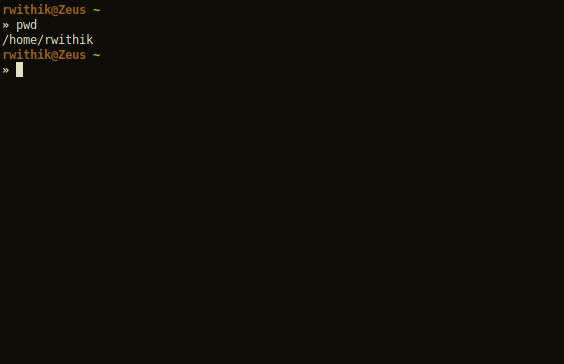
\includegraphics[scale=.5]{../Images/Cycle2/1.png}\newline
\newline
Question 2: Change to /etc directory.\newline
Output:\newline
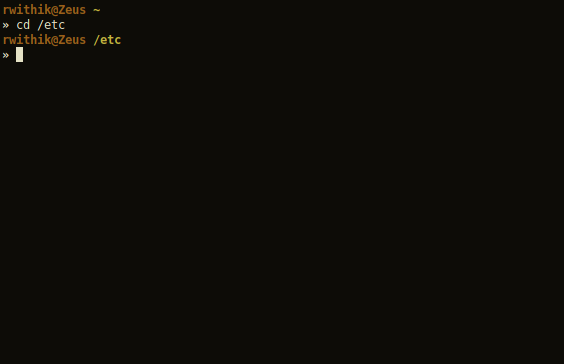
\includegraphics[scale=.5]{../Images/Cycle2/2.png}
\pagebreak
\newline
Question 3: Change to home directory using a single command.\newline
Output:\newline
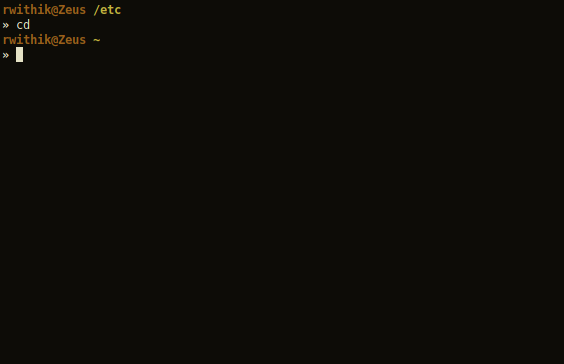
\includegraphics[scale=.5]{../Images/Cycle2/3.png}\newline
\newline
Question 4: Change to the parent directory of the current directory.\newline
Output:\newline
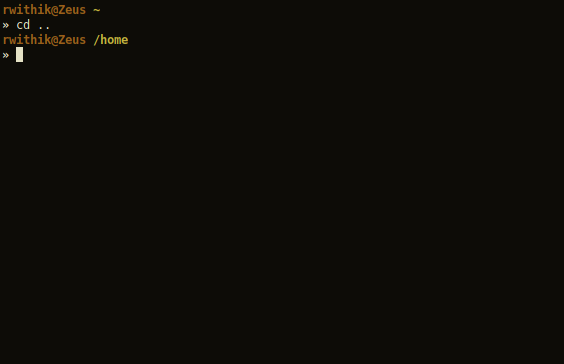
\includegraphics[scale=.5]{../Images/Cycle2/4.png}
\pagebreak
\newline
Question 5: Go to the root directory.\newline
Output:\newline
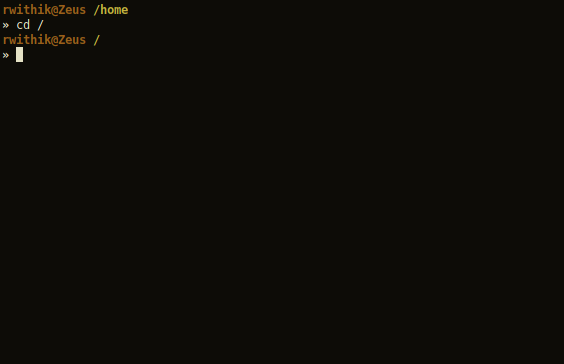
\includegraphics[scale=.5]{../Images/Cycle2/5.png}\newline
\newline
Question 6: Give a long listing of the root directory.\newline
Output:\newline
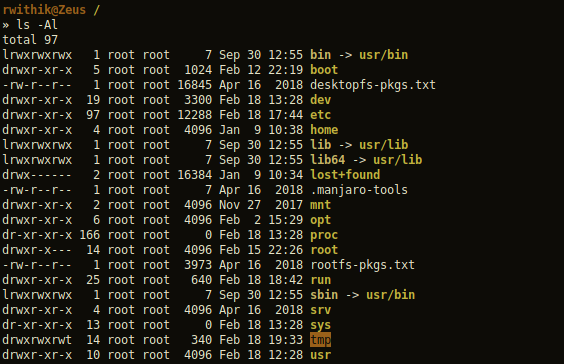
\includegraphics[scale=.5]{../Images/Cycle2/6.png}\pagebreak
\newline
Question 7: Give a listing of the last 10 files of the root directory.\newline
Output:\newline
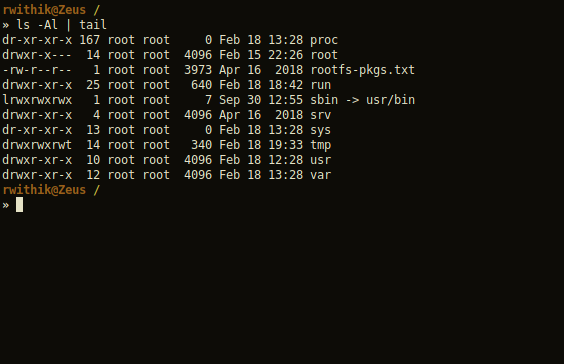
\includegraphics[scale=.5]{../Images/Cycle2/7.png}\newline
\newline
Question 8: Stay where you are, and list the contents of /etc.\newline
Output:\newline
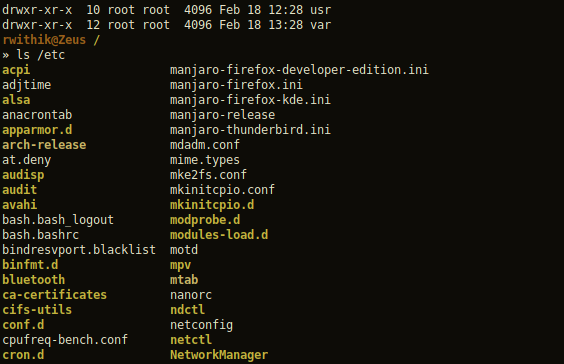
\includegraphics[scale=.5]{../Images/Cycle2/8.png}\pagebreak
\newline
Question 9: Create a directory testdir in your home directory.\newline
Output:\newline
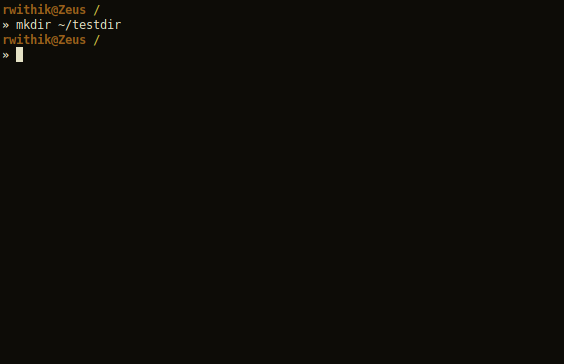
\includegraphics[scale=.5]{../Images/Cycle2/9.png}\newline
\newline
Question 10: Change to the /etc directory, stay there and create a directory newdir in your home
directory(using a single command).\newline
Output:\newline
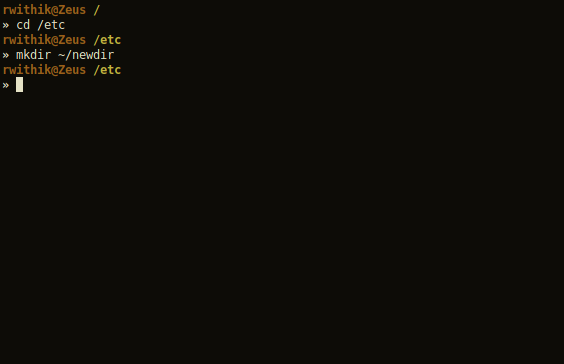
\includegraphics[scale=.5]{../Images/Cycle2/10.png}\pagebreak
\newline
Question 11: Create in one command the directories ~/dir1/dir2/dir3 (dir3 is a subdirectory from dir2,and dir2 is a subdirectory from dir1).\newline
Output:\newline
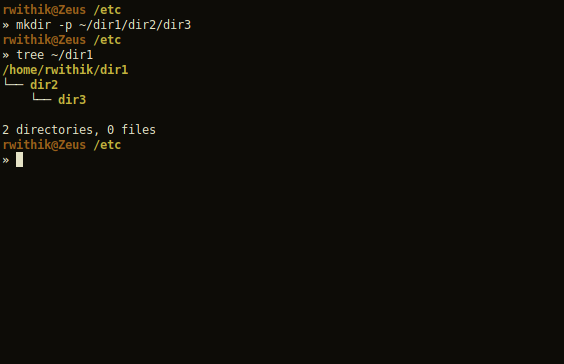
\includegraphics[scale=.5]{../Images/Cycle2/11.png}\newline
\newline
Question 12: Display the calendar for April 2019.\newline
Output:\newline
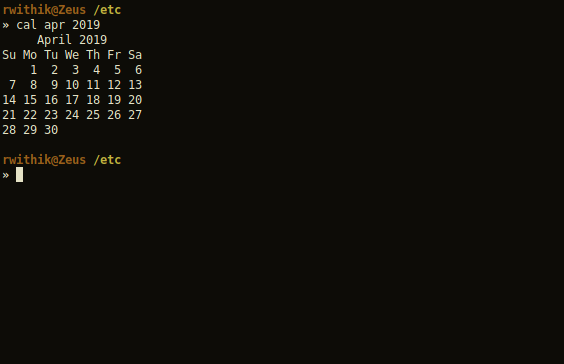
\includegraphics[scale=.5]{../Images/Cycle2/12.png}\pagebreak
\newline
Question 13: Display that ‘There are ......... files in my current directory’ . The ......... should be filled with the count of the files.\newline
Output:\newline
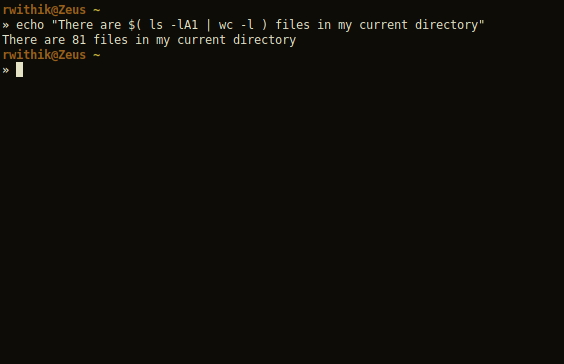
\includegraphics[scale=.5]{../Images/Cycle2/13.png}\newline
\newline
Question 14: List all the files (including hidden files) in your home directory.\newline
Output:\newline
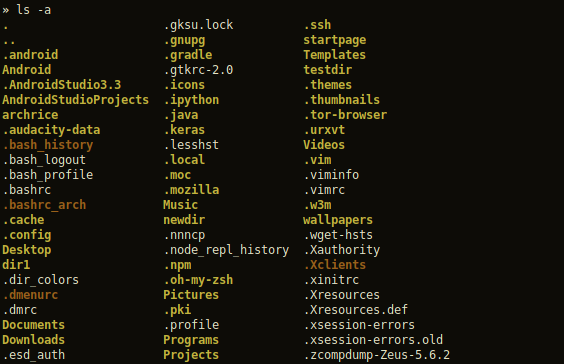
\includegraphics[scale=.5]{../Images/Cycle2/14.png}\pagebreak
\newline
Question 15: Redirect the output of the above command to a new file FileList.txt.\newline
Output:\newline
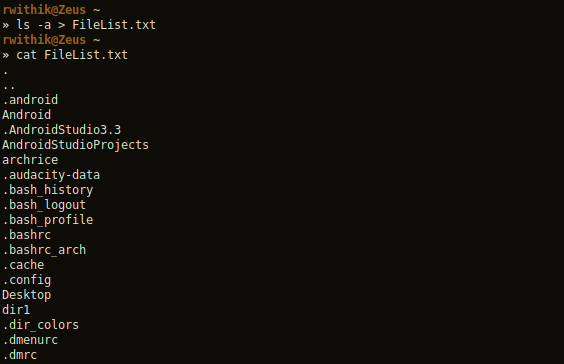
\includegraphics[scale=.5]{../Images/Cycle2/15.png}\newline
\newline
Question 16: Redirect the number of lines of FileList.txt to CountFile.txt.\newline
Output:\newline
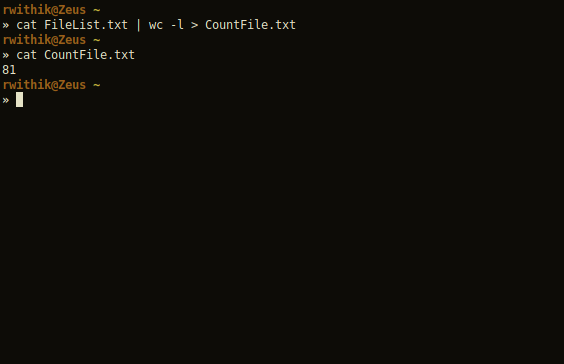
\includegraphics[scale=.5]{../Images/Cycle2/16.png}\pagebreak
\newline
Question 17: List all the files in your home directory starting with ‘s’ .\newline
Output:\newline
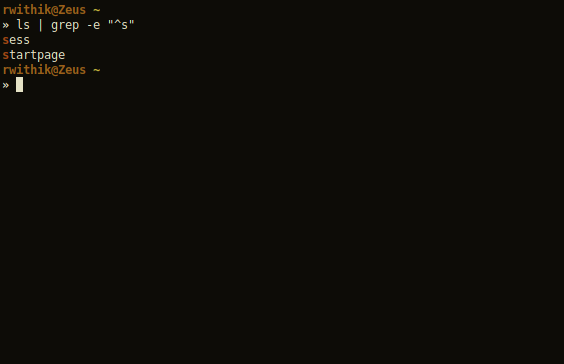
\includegraphics[scale=.5]{../Images/Cycle2/17.png}\newline
\newline
Question 18: List all the file-names starting with “a”, “b” or “s” .\newline
Output:\newline
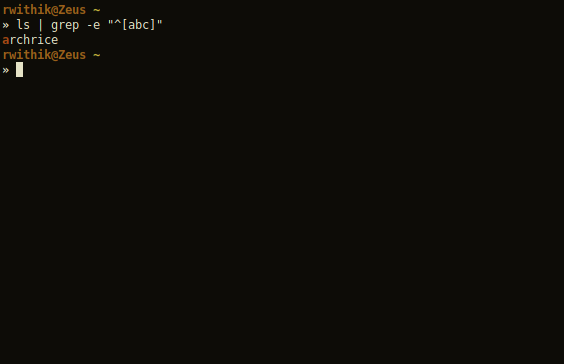
\includegraphics[scale=.5]{../Images/Cycle2/18.png}\pagebreak
\newline
Question 19: Create two files ‘Countries.txt’, containing country names and their corresponding capital cities and ‘Story.txt’ contains some arbitrary lines of text.\newline
Output:\newline
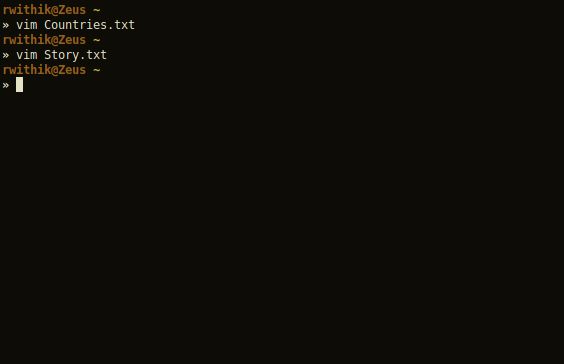
\includegraphics[scale=.5]{../Images/Cycle2/19A.png}\newline
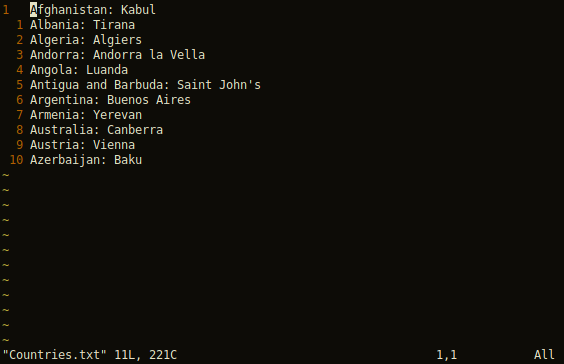
\includegraphics[scale=.5]{../Images/Cycle2/19B.png}\newline
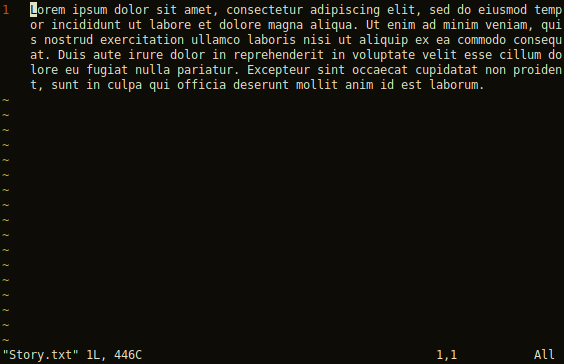
\includegraphics[scale=.5]{../Images/Cycle2/19C.png}\newline
\newline
Question 20: Convert all lowercase characters from ‘Story.txt’ to uppercase and store it in a file ‘Capstory.txt’.\newline
Output:\newline
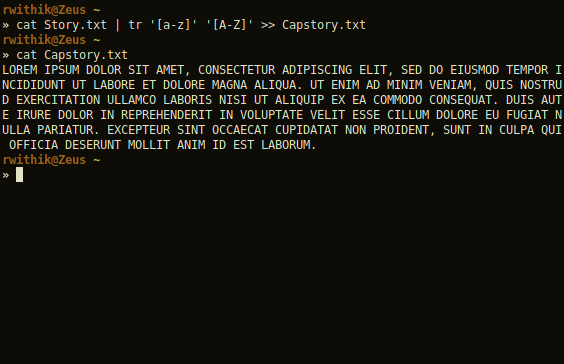
\includegraphics[scale=.5]{../Images/Cycle2/20.png}\pagebreak
\newline
Question 21: Toggle the cases in ‘Story.txt’ and store it in a file ‘Togglestory.txt’.\newline
Output:\newline
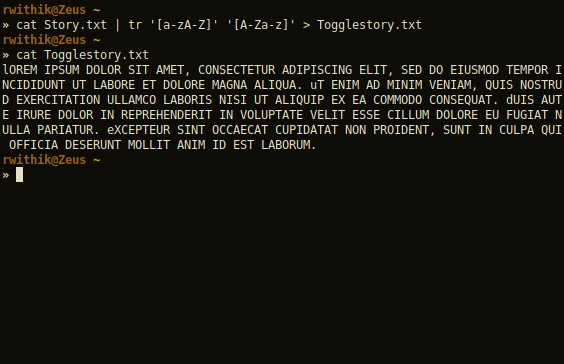
\includegraphics[scale=.5]{../Images/Cycle2/21.png}\newline
\newline
Question 22: Sort the contents of ‘Countries.txt’with Capital as the primary sort key and write the sorted output to ‘SortCountry.txt’.\newline
Output:\newline
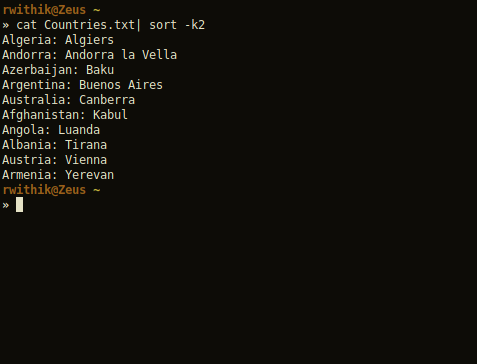
\includegraphics[scale=.5]{../Images/Cycle2/22.png}\pagebreak
\newline
Question 23: Display only the capital cities from ‘Countries.txt’.\newline
Output:\newline
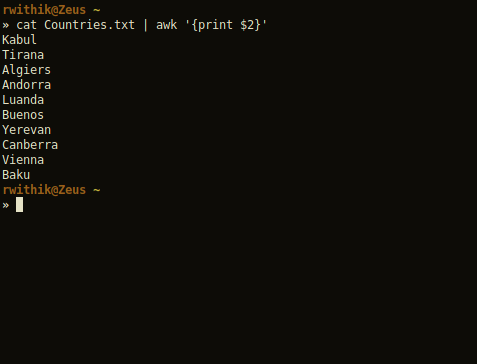
\includegraphics[scale=.5]{../Images/Cycle2/23.png}\newline
\newline
Question 24: Locate all ‘.txt’ and ‘.doc’ files in the current directory .\newline
Output:\newline
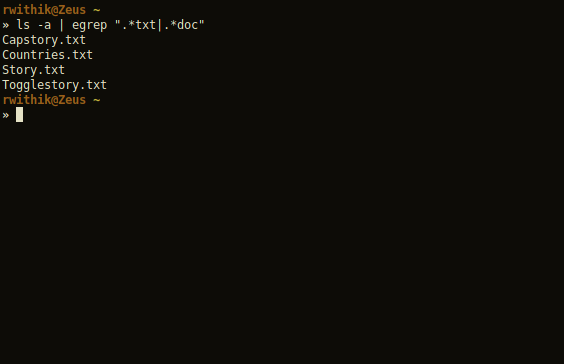
\includegraphics[scale=.5]{../Images/Cycle2/24.png}\pagebreak
\newline
Question 25: Count the number of occurence of ‘the’ in ‘Story.txt’.\newline
Output:\newline
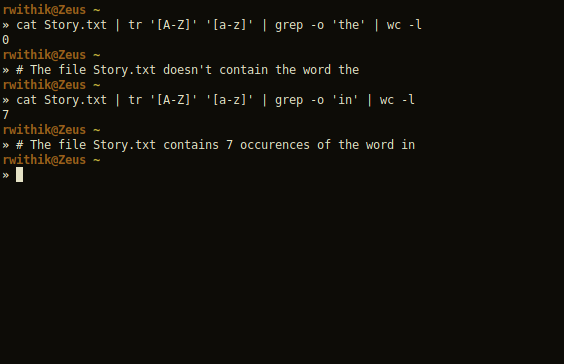
\includegraphics[scale=.5]{../Images/Cycle2/25.png}\newline
\newline
\end{document}
